\documentclass{article}

\usepackage[spanish]{babel}
\usepackage[utf8]{inputenc}
\usepackage[margin=3cm]{geometry}
\usepackage[font=footnotesize,labelfont=bf]{caption}
\usepackage{float}
\usepackage{framed}
\usepackage{color}
\usepackage{wrapfig}\definecolor{shadecolor}{RGB}{224,238,238}
\usepackage{listings}
\usepackage{tikz}
\usepackage{enumitem}
\usepackage{xcolor}

\graphicspath{{images/}}

\title{Trabajo Practico 3: Implementación BIP - Basic Instruction Set Processor}
\author{Perez, Federico\\
        \texttt{perezfederico@unc.edu.ar}
        \and
        Sardoy, Juan Manuel\\
        \texttt{jmsardoy@gmail.com}
        }
\begin{document}

\maketitle
\begin{center}
    
\includegraphics[scale=2]{unc-logo}
\end{center}
\newpage
\section{Descripción del trabajo}

\indent El siguiente trabajo consiste en la implementación práctica de un procesador de propósito educativo
llamado BIP, o Basic Instruction Set Processor. Dicho procesador, tiene la característica de ser muy simple
y de facil entendimiento, lo que facilita el aprendizaje de arquitecturas de computadoras de propósito general. \\
\indent Es un diseño monociclo, con división de memoria y de canales de datos e instrucciones. En las siguientes secciones se explicaran los detalles de la arquitectura con mas profundidad. \\
\indent La estructura final de la presentación constará del BIP sintetizado en una FPGA, que se debera comunicar
mediante una interfaz, al modulo UART implementado en el Trabajo Práctico número 2, también sintetizado en dicha FPGA,
que luego mediante un conversor UART/USB, se comunicará con un software corriendo en una computadora personal.
Dentro de la memoria de programa del BIP, deberá existir de forma estática, un programa que ejecute una secuencia de
operaciones matemáticas a elección del implementador. Dicho programa debera iniciar su ejecución, cuando desde la computadora,  se envíe un comando de arranque. Luego, el software en la computadora deberá esperar que el BIP
termine su ejecución y este deberá enviar el resultado por UART, para ser mostrado por pantalla. \\

\indent En cuanto a políticas de trabajo, se tratará de llevar a cabo una implementación muy modular y parametrizada del BIP. Esto se verá reflejado en la cantidad de archivos de \textit{headers} y parámetros aceptados por cada uno de los módulos. Se evitaran los famosos \textit{magic numbers}, para darle un grado lo más profesional posible al código. \\
\newpage
\section{Arquitectura general}
\indent Como se mencionó anteriormente, se trata de un procesador monociclo,
osea que ejecuta una instrucción por ciclo. Esto trae aparejado el impedimento lógico fundamental de que,
para que una instrucción sea ejecutada , todo el proceso desde que se obtiene la instrucción de la memoria,
hasta su ejecución, debe transcurrir entre dos flancos de clock. Esto límita mucho la velocidad del procesador,
dado que la velocidad del clock esta atada inversamente al tiempo de propagación logica entre los circuitos combinacionales.
Tampoco se puede crear un complejo diseño dado que esto reduciría mas la performance por el mismo motivo.

\begin{figure}[H]
    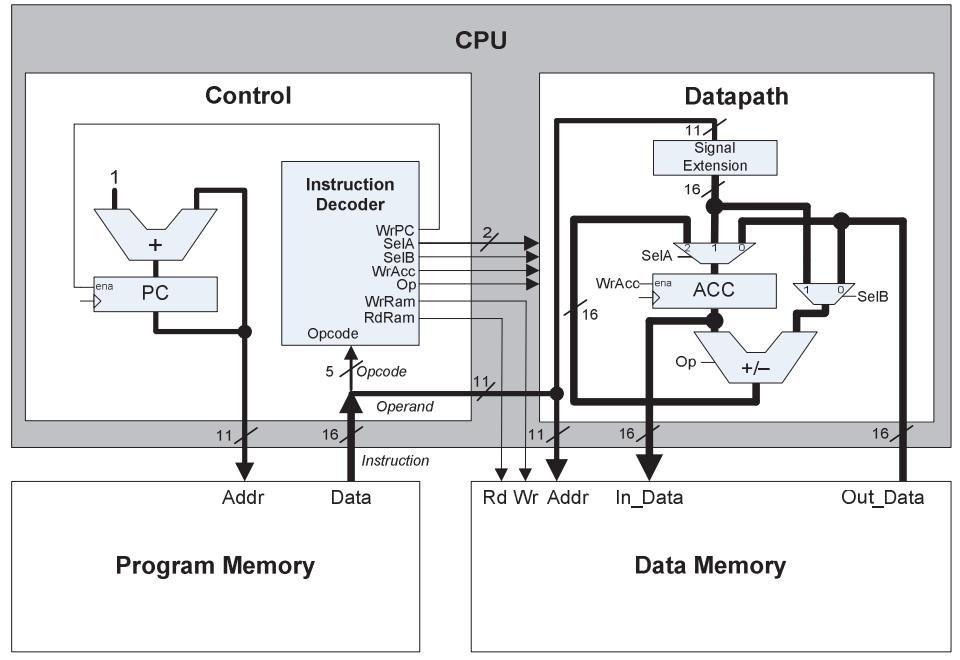
\includegraphics[scale=0.5]{bip_arch}
    \caption{\textit{Diagrama de la arquitectura básica del BIP}}
\end{figure}

Podemos observar claramente los dos bloques principales.
\indent El primero, llamado bloque de \textit{Control}, es el que se encarga de decodificar
la intrucción recibida desde la memoria de programa, y controlar las diferentes señales que operan el resto
del procesador. \\
\indent El segundo, llamado \textit{datapath} o bloque de datos, es el que se conecta con la memoria de datos y ejecuta las operaciones indicadas por el bloque de control. \\ \\

El bloque de control recibe los cinco bits más significativos de cada instruccíon (también llamados \textit{opcode}),
los cuales indican qué instrucción se desea ejecutar.

\begin{figure}[H]
    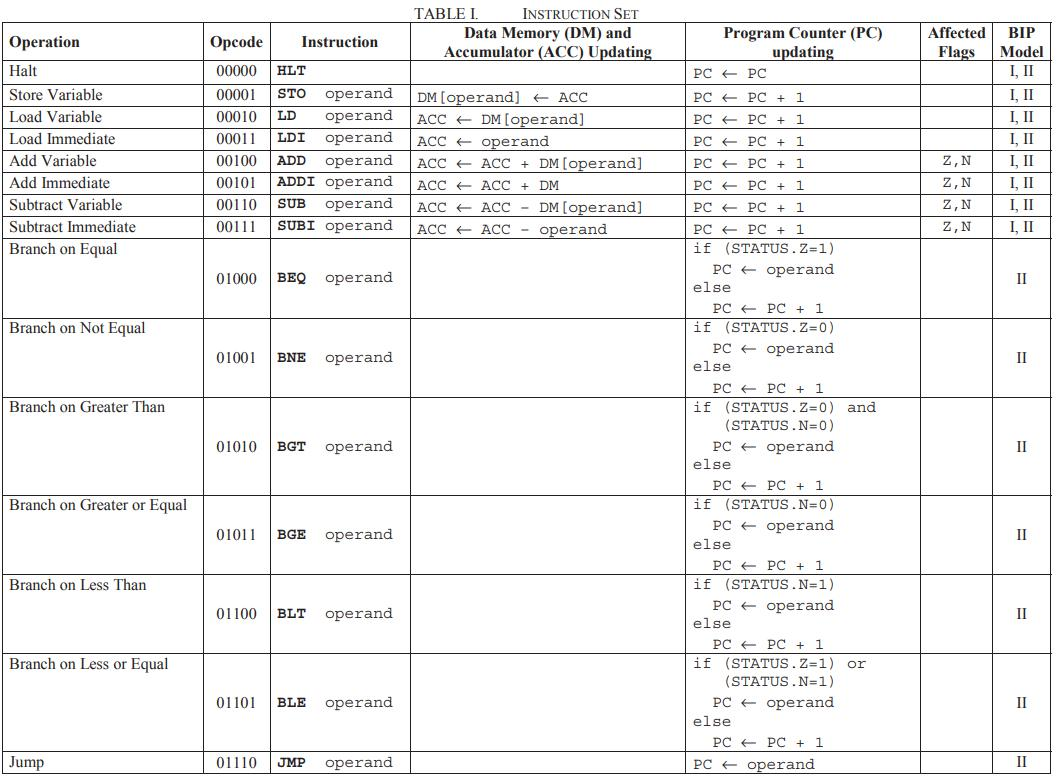
\includegraphics[scale=0.5]{opcodes}
    \caption{\textit{Instrucciones soportadas por el BIP y sus respectivas acciones ejecutadas}}
\end{figure}

Cabe destacar, que dada la consigna del trabajo práctico, no serán implementadas las intrucciones de saltos,
ya sean condicionales o no, con el motivo de hacer mas facil la implementación practica del procesador.
Sin embargo se verá mas adelante, que incluir dichas instrucciones en la implementación es trivial, dado
el diseño modular que se penso para cada parte del sistema.

\newpage
\section{Implementación}

A continuación se detallará la lógica seguida y su implementación en el lenguaje de descripción de hardware Verilog,
para cada módulo del BIP.

\subsection{Memoria de programa}

La memoria de programa es simplemente un arreglo de registros con datos fijos, siendo estos, el programa
\textit{"hardcodeado"} a ejecutar. A continuación, su implementación en Verilog:

\begin{shaded}
\begin{lstlisting}[language=Verilog]
`include "memory_defs.vh"

module ProgramMemory
#(
    parameter ADDRESS_BITS = `ADDRESS_BITS,
    parameter DATA_BITS = `DATA_BITS
)
(
    input clk,
    input rst,
    input wire [ADDRESS_BITS-1:0] i_address,
    output reg [DATA_BITS-1:0] o_data
);

    localparam MEM_SIZE = 2**ADDRESS_BITS;

    reg [DATA_BITS-1:0] mem [0:MEM_SIZE-1];

    `define INSTRUCTION(MNEMONIC, OPCODE) localparam MNEMONIC = OPCODE;
    `include "instructions.vh"

    always@(posedge clk) begin
        if(!rst) begin

            `define                                     \
            DATA_MEMORY(ADDRESS, MNEMONIC, ARGS)        \
                mem[ADDRESS] <= {MNEMONIC, ARGS};

            `include "program.vh"

            //para evitar warning que elimina bits de o_data
            mem[`LAST_ADDRESS] <= {16{1'b1}};
            o_data  <= {16{1'b1}};
        end
        else begin
            o_data <= mem[i_address];
        end
    end

endmodule
\end{lstlisting}
\end{shaded}

Como se ve en el código, también en la definicion de las intrucciones y sus
\textit{opcodes} se utilizo la técnica de X-Macro.

En el archivo \textit{instructions.vh} se observa la definición de todas las instrucciones
definidas por el "standard" del BIP, restando las instrucciones no implementadas, como
se mencionó anteriormente.

\begin{shaded}
\begin{lstlisting}
`ifndef INSTRUCTIONS_VH
`define INSTRUCTIONS_VH

`INSTRUCTION(HLT, 'b00000)
`INSTRUCTION(LD,  'b00010)
`INSTRUCTION(LDI, 'b00011)
`INSTRUCTION(ADD, 'b00100)
`INSTRUCTION(ADDI,'b00101)
`INSTRUCTION(SUB, 'b00110)
`INSTRUCTION(STO, 'b00001)
`INSTRUCTION(SUBI, 'b00111)

`undef INSTRUCTION

`endif
\end{lstlisting}
\end{shaded}

\newpage

Podemos observar que el programa se inserta dentro de la memoria mediante la técnica conocida como \textit{X-Macro}. \\
Esta técnica implia definir una macro para tareas repetitivas, y luego en otro archivo, el cual
será utilizado en el lugar correspondiente, hará uso de dicha macro, listando todos los elementos deseados.
Esto facilita la "programación" y la tarea de debugging, y también reduce la posibilidad de errores,
dado que el mismo tiene una sintáxis mucho mas simple y se encuentra incluido en otro archivo fuente.
Tambien mejora la prolijidad del código, al separar la lógica y datos. \\

Esta tecnica se aplicará en varios lugares a lo largo del proyecto.

El archivo \textit{program.vh} entonces, contendrá el programa propiamente dicho:

\begin{shaded}
\begin{lstlisting}[language=Verilog]
`ifndef PROGRAM_VH
`define PROGRAM_VH

`DATA_MEMORY(0, LDI,  -11'd4)
`DATA_MEMORY(1, STO,   11'd1)
`DATA_MEMORY(2,  LDI,  11'd2)
`DATA_MEMORY(3,  ADD,  11'd1)
`DATA_MEMORY(4,  STO,  11'd2)
`DATA_MEMORY(5,  LDI,  11'd123)
`DATA_MEMORY(6,  ADDI, 11'd7)
`DATA_MEMORY(7,  LD,   11'd2)
`DATA_MEMORY(8,  ADDI, 11'd4)
`DATA_MEMORY(9,  SUBI, 11'd50)
`DATA_MEMORY(10, SUB,  11'd1)
`DATA_MEMORY(11, HLT,  11'd0)

`undef DATA_MEMORY

`endif
\end{lstlisting}
\end{shaded}


El programa realiza una serie de operaciones aritméticas y de transacciones de memoria
(hace uso de todas las instrucciones implementadas), y luego se detiene con la instruccion \textit{HLT o HALT}.

\newpage

\subsection{Memoria de datos}

La memória de datos sigue una lógica muy similar a la de programa, con la salvedad de que la última tiene
un tamaño fijo y vacío. No se cuenta con una memoria con datos iniciales. Todos los datos que se deseen
guardar deben ser guardados en tiempo de ejecución y mediante software. La instrucción para guardar un dato
es \textit{STR o STORE} y para cargarlo es \textit{LD o LDI.}

El código de Verilog para el módulo de la memoria de datos es el siguiente:

\begin{shaded}
\begin{lstlisting}[language=Verilog]
`include "memory_defs.vh"

module DataMemory
#(
    parameter ADDRESS_BITS = `ADDRESS_BITS,
    parameter DATA_BITS = `DATA_BITS
)
(
    input clk,
    input read,
    input write,
    input wire [ADDRESS_BITS-1:0] i_address,
    input wire [DATA_BITS-1:0] i_data,
    output reg [DATA_BITS-1:0] o_data
);

    localparam MEM_SIZE = 2**ADDRESS_BITS;

    reg [DATA_BITS-1:0] mem [0:MEM_SIZE-1];

    always@(negedge clk)
    begin
        if (read)
        begin
            o_data <= mem[i_address];
        end
        else if (write)
        begin
            mem[i_address] <= i_data;
        end
    end
endmodule
\end{lstlisting}
\end{shaded}

\newpage

\subsection{Bloque de Control}

El bloque de control implementa la lógica de decodificación y control de cada una de las instrucciones,
como asi también el Program Counter Pointer o PC. El módulo controla todos los elementos, del módulo de datos. \\
Algunos de los controles que posee son:

\begin{description}[font=$\bullet$~\normalfont\scshape\color{red!50!black}]
\item Habilitar el contador de programa, para que comience a contar.
\item Elegir fuente del registro A y B que van a la ALU. Las fuentes del A pueden ser
memoria, extensor de signo, o realimentación de la ALU misma. Los del B puede ser de
memoria o del extensor de signo. El extensor de signo se explicará en la sección del bloque
datos.
\item Habilitar la escritura del acumulador. El acumulador es un latch que guarda el dato de
entrada con cada ciclo de clock, cuando su señal habilitadora esta en alto.
\item Elegir la operación a efectuar por la ALU. En este caso solamente puede sumar o restar.
\item Leer o escribir RAM. Habilita la RAM de datos para lectura o escritura. Si esta en lectura,
los datos en la dirección de memoria seleccionada por el bus de direcciones, saldran por la salida
de datos. Si esta en escritura, los datos a la salida del acumulador, serán escritos en la dirección
de memoria seleccionada por el bus de direcciones.

\newpage

A continuación, la implementación práctica del bloque de control:

\begin{shaded}
\begin{lstlisting}[language=Verilog]
`include "memory_defs.vh"

module Control
#(
    parameter ADDRESS_BITS = `ADDRESS_BITS,
    parameter DATA_BITS = `DATA_BITS
)
(
    input clk,
    input rst,
    input [DATA_BITS - 1:0] i_instruction,
    output [ADDRESS_BITS - 1 : 0] o_prog_address,
    output [ADDRESS_BITS - 1 : 0] o_operand,
    output [ 1 : 0] o_sel_a,
    output o_sel_b,
    output o_write_acc,
    output o_operation,
    output o_write_mem,
    output o_read_mem,
    output o_done
);

    wire enable_pc;

    wire [4 : 0] opcode = i_instruction[DATA_BITS - 1:ADDRESS_BITS];
    assign o_operand = i_instruction[ADDRESS_BITS - 1:0];

    reg [10 : 0] program_counter;

    always@(negedge clk) begin
        if (!rst) begin
            program_counter <= 0;
        end
        else begin
            if (enable_pc) begin
                program_counter <= program_counter+1;
            end
        end
    end

    assign o_prog_address = program_counter;

    InstructionDecoder ID_u
    (
        .opcode(opcode),
        .o_enable_pc(enable_pc),
        .o_sel_a(o_sel_a),
        .o_sel_b(o_sel_b),
        .o_write_acc(o_write_acc),
        .o_operation(o_operation),
        .o_write_mem(o_write_mem),
        .o_read_mem(o_read_mem),
        .bip_done(o_done)
    );


endmodule
\end{lstlisting}
\end{shaded}
\end{description}

Como se observa, la lógica del módulo de control es puramente combinacional, con excepción del
PC, el cual es un registro que se le suma una unidad en cada ciclo de clock.

\newpage

\subsection{Bloque de datos}

El bloque de datos es el módulo mas complejo del BIP. Es el que se encarga del procesamiento y operatoria
intrinsecas del procesador.\\

\noindent Sus submódulos son:
\begin{description}[font=$\bullet$~\normalfont\scshape\color{red!50!black}]
\item [Extensor de signo] El extensor de signo es un módulo que extiende de un registro
de 11 bits con signo, a uno de 16 bits con signo. Sirve para extender los datos inmediatos, osea
los que vienen desde la instrucción misma (los cuales son de 11 bits) al largo del registro de
operación del BIP, el cual es 16 bits.
\item [Selector A] Selecciona la fuente de entrada de los datos para el acumulador. Como se explicó
anteriormente, las fuentes posibles son: desde la \textit{memoria de datos}, el \textit{extensor de signo} y la \textit{ALU}.
\item [Selector B] Selecciona la fuente de entrada de datos para el segundo operando de la ALU.
Las fuentes posibles son: desde la \textit{memoria de datos} y desde el \textit{extensor de signo}.
\item [Acumulador] Es un \textit{latch} que funciona a modo de registro de propósito general del
procesador. Se pueden acumular resultados para ser utilizados en las siguientes instrucciones. Es controlado mediante su pin de habilitación. Cuando esta en alto, a su salida, muestra los datos de la entrada, luego del flanco de clock. Su salida se utiliza tanto para entrada a la ALU, como para entrada
de memoria de datos.
\item [ALU] Circuito combinacional encargado de realizar las operación matemáticas y lógicas del procesador. En el caso del BIP, las únicas operaciones que realiza son de suma y resta. Se controla
unicamente mediante un pin selector de operación, y mediante los operandos A y B, los cuales contienen
los argumentos de dichas operaciones.
\end{description}

\noindent La implementación del módulo de datos es la siguiente:

\begin{shaded}
\begin{lstlisting}[language=Verilog]
`include "memory_defs.vh"

module Datapath
#(
    parameter ADDRESS_BITS = `ADDRESS_BITS,
    parameter DATA_BITS = `DATA_BITS
)
(
    input  clk,
    input  rst,
    input  [ADDRESS_BITS - 1 : 0] i_operand,
    input  [ 1 : 0] i_sel_a,
    input  i_sel_b,
    input  i_write_acc,
    input  i_operation,
    input  [DATA_BITS - 1 : 0] i_mem_data,
    output [DATA_BITS - 1 : 0] o_mem_data,
    output [ADDRESS_BITS - 1 : 0] o_mem_address
);

    reg  signed [DATA_BITS - 1 : 0] accumulator;
    wire signed [DATA_BITS - 1 : 0] op_result;
    wire signed [DATA_BITS - 1 : 0] operand_ext;
    wire signed [DATA_BITS - 1 : 0] multiplexor_b;


    //multiplexor b
    assign multiplexor_b = (i_sel_b) ? operand_ext : i_mem_data;

    //signal extention
    assign operand_ext =
    {{(DATA_BITS - ADDRESS_BITS){i_operand[ADDRESS_BITS - 1]}}, i_operand};

    //operation unit
    assign op_result = (i_operation) ? accumulator - multiplexor_b
                                     : accumulator + multiplexor_b;

    always@(posedge clk) begin
        if(!rst) begin
            accumulator <= 0;
        end
        else begin
            if (i_write_acc) begin
                case(i_sel_a)
                    0: accumulator <= i_mem_data;
                    1: accumulator <= operand_ext;
                    2: accumulator <= op_result;
                    default: accumulator <= 0;
                endcase
            end
            else begin
                accumulator <= accumulator;
            end
        end
    end

    assign o_mem_address = i_operand;
    assign o_mem_data = accumulator;

endmodule
\end{lstlisting}
\end{shaded}

Si bien es el módulo más complejo analizado hasta ahora, no es de gran dificultad entender
su funcionamiento. El BIP en general esta pensado para ser de facil implementación.

\newpage

\subsection{Interfaz}

La interfaz es el módulo que se encarga de interpretar los comandos recibidos desde la computadora
por UART, e indicar las operaciones correspondientes al BIP. En este caso, la interfaz espera una señal
para arrancar el procesador, y por ende el programa fijo dentro de la memoria de programa. Una vez que
el programa termina (cuando se detecta que la instrucción HALT ha sido ejecutada), se envía el resultado
del acumulador hacia el usuario en la computadora. Es un módulo simple pero nos sirve para ver y entender
el funcionamiento del BIP. \\

Está implementado mediante una pequeña máquina de estados:

\begin{shaded}
\begin{lstlisting}
`include "memory_defs.vh"

module Interface
#(
    parameter ADDRESS_BITS = `ADDRESS_BITS,
    parameter DATA_BITS = `DATA_BITS
)
(
    input clk,
    input rst,
    input [DATA_BITS - 1 : 0] accumulator,
    input [7 : 0] inst_count,
    input bip_done,
    output o_tx
);

    wire baud_rate;
    wire tx_done;

    reg tx_start;
    reg [7 : 0] tx_data;

    reg next_tx_start;
    reg [7 : 0] next_tx_data;

    reg [3 : 0] state;
    reg [3 : 0] next_state;

    reg [DATA_BITS -1: 0] accumulator_latch;
    reg [ 7 : 0] inst_count_latch;
    reg [DATA_BITS -1 : 0] next_accumulator_latch;
    reg [ 7 : 0] next_inst_count_latch;


    localparam IDLE = 0;
    localparam SEND_INST_COUNT = 1;
    localparam WAIT1 = 2;
    localparam WAIT11 = 3;
    localparam SEND_ACC_HIGH = 4;
    localparam WAIT2 = 5;
    localparam WAIT22 = 6;
    localparam SEND_ACC_LOW = 7;
    localparam WAIT3 = 8;
    localparam WAIT33 = 9;
    localparam STOP = 10;

    always@(posedge clk) begin
        if(!rst) begin
            state <= 0;
            tx_start <= 0;
            tx_data <= 0;
            accumulator_latch <= 0;
            inst_count_latch <= 0;
        end
        else begin
            state <= next_state;
            tx_start <= next_tx_start;
            tx_data <= next_tx_data;
            accumulator_latch <= next_accumulator_latch;
            inst_count_latch <= next_inst_count_latch;
        end
    end


    always@* begin
        next_state = state;
        next_tx_start = 0;
        next_tx_data = tx_data;
        next_accumulator_latch = accumulator_latch;
        next_inst_count_latch = inst_count_latch;

        case(state)
            IDLE:
            begin
                if(bip_done) begin
                    next_accumulator_latch = accumulator;
                    next_inst_count_latch = inst_count;
                    next_state = SEND_INST_COUNT;
                end
            end

            SEND_INST_COUNT:
            begin
                next_tx_data = inst_count_latch;
                next_tx_start = 1;
                next_state = WAIT1;
            end

            WAIT1:
            begin
                next_state = WAIT11;
            end

            WAIT11:
            begin
                if(tx_done) next_state = SEND_ACC_HIGH;
            end

            SEND_ACC_HIGH:
            begin
                next_tx_data = accumulator_latch[15:8];
                next_tx_start = 1;
                next_state = WAIT2;
            end

            WAIT2:
            begin
                next_state = WAIT22;
            end

            WAIT22:
            begin
                if(tx_done) next_state = SEND_ACC_LOW;
            end

            SEND_ACC_LOW:
            begin
                next_tx_data = accumulator_latch[7:0];
                next_tx_start = 1;
                next_state = WAIT3;
            end

            WAIT3:
            begin
                next_state = WAIT33;
            end

            WAIT33:
            begin
                if(tx_done) next_state = STOP;
            end

            STOP:
            begin
                next_state = STOP;
            end

        endcase
    end

    TX tx_u
    (
        .clk(clk),
        .rst(rst),
        .i_baud_rate(baud_rate),
        .i_tx_start(tx_start),
        .i_data(tx_data),
        .o_tx_done(tx_done),
        .o_tx(o_tx)
    );

    BaudRateGenerator baud_rate_u
    (
        .clk(clk),
        .rst(rst),
        .out(baud_rate)
    );
endmodule
\end{lstlisting}
\end{shaded}


\newpage
\end{document}
